%%%%%%%%%%%%%%%%%%%%%%%%%%%%%%%%%%%%%%%%%
% NIH Grant Proposal for the Specific Aims and Research Plan Sections
% LaTeX Template
% Version 1.0 (21/10/13)
%
% This template has been downloaded from:
% http://www.LaTeXTemplates.com
%
% Original author:
% Erick Tatro (erickttr@gmail.com) with modifications by:
% Vel (vel@latextemplates.com)
% Michael ma2196@columbia.edu
% with assistance from Jonah G.
% Adapted from:
% J. Hrabe (http://www.magalien.com/public/nih_grants_in_latex.html)
%
% License:
% CC BY-NC-SA 3.0 (http://creativecommons.org/licenses/by-nc-sa/3.0/)
%
%%%%%%%%%%%%%%%%%%%%%%%%%%%%%%%%%%%%%%%%%

%----------------------------------------------------------------------------------------
%	PACKAGES AND OTHER DOCUMENT CONFIGURATIONS
%----------------------------------------------------------------------------------------

\documentclass[11pt,notitlepage]{article}

% A note on fonts: As of 2013, NIH allows Georgia, Arial, Helvetica, and Palatino Linotype. LaTeX doesn't have Georgia or Arial built in; you can try to come up with your own solution if you wish to use those fonts. Here, Palatino & Helvetica are available, leave the font you want to use uncommented while commenting out the other one.

\usepackage[super]{natbib}
\usepackage{palatino} % Palatino font
%\usepackage{helvet} % Helvetica font
\renewcommand*\familydefault{\sfdefault} % Use the sans serif version of the font
\usepackage[T1]{fontenc}
\linespread{1.05} % A little extra line spread is better for the Palatino font
\usepackage{bibentry} % needed to use \nobibiography to omit the bibliography at the end.
\usepackage{hyperref} % to allow hyperlinks to websites on the internet
\usepackage[hypcap]{caption} % to point to the top of the image
\usepackage{lipsum} % Used for inserting dummy 'Lorem ipsum' text into the template
\usepackage{amsfonts, amsmath, amsthm, amssymb} % For math fonts, symbols and environments
\usepackage{graphicx} % Required for including images
\usepackage{booktabs} % Top and bottom rules for table
\usepackage{wrapfig} % Allows in-line images
\usepackage[labelfont=footnotesize]{caption} % Make figure numbering in captions bold
\usepackage[top=0.5in,bottom=0.5in,left=0.5in,right=0.5in]{geometry} % Reduce the size of the margin
\pagestyle{empty} % Remove page numbers

\hyphenation{ionto-pho-re-tic iso-tro-pic fortran} % Specifies custom hyphenation points for words or words that shouldn't be hyphenated at all

  
  % to reduce white space between PARAGRAPHS
\setlength{\parskip}{-4pt}
\setlength{\parsep}{0pt}

  % additional parameters
%\setlength{\headsep}{0pt}
%\setlength{\topskip}{0pt}
%\setlength{\topmargin}{0pt}
%\setlength{\topsep}{0pt}
%\setlength{\partopsep}{0pt}

  % to reduce white space around figures
% \setlength{\textfloatsep}{0pt plus 0pt minus 0pt}

  % to reduce white space between SECTIONS
\usepackage[compact]{titlesec}
\titlespacing{\part}{0pt}{5pt}{4pt}
%\titlespacing{\subsection}{0pt}{*0}{*0}
%\titlespacing{\subsubsection}{0pt}{*0}{*0}
%\titlespacing{\subparagraph}{0pt}{*0}{*0}
\titlespacing*{\subparagraph} {\parindent}{1ex plus 1ex minus .2ex}{0.5em}


\begin{document} 
%----------------------------------------------------------------------------------------
%	RESEARCH PLAN
%----------------------------------------------------------------------------------------
\section*{Research Plan}

\subsection*{A. Significance}

\subsection*{Respiratory failure in hospitalized patients can be predicted and should be prevented.} 

\begin{wrapfigure}{R}{6.cm}
 \vspace{-10pt}
 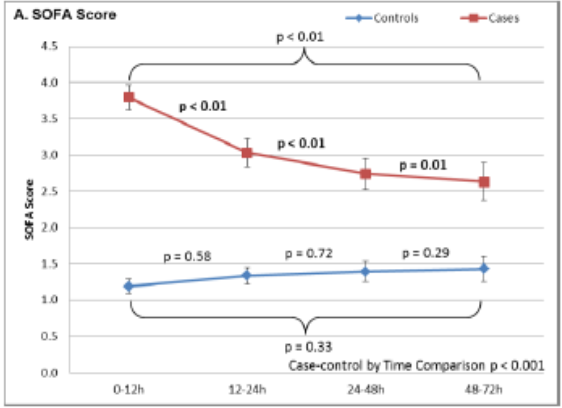
\includegraphics[scale=0.7]{Figures/SOFA_fig.png}
  \vspace{-25pt}
  \caption{\footnotesize Deterioration of the Sequential Organ Failure Assessment score (SOFA) can be detected 24-48 hours before clinical deterioration leads to ICU admission; p-values reflect pair-wise comparisons between consecutive time intervals, adjusting for patient characteristics. \cite{Yu_24970344}.}
    \label{fig:SOFA_fig}
 \vspace{-15pt}
\end{wrapfigure}

Acute respiratory failure (ARF) requiring mechanical ventilation is common in hospitalized patients, consuming a disproportionate amount of health care resources in the USA \cite{Wunsch_20639743}. Short term mechanical ventilation can be life saving, but prolonged mechanical ventilation often leads to multi-organ failure and death \cite{Wunsch_20639743, Ranieri_10872010}. Most research focuses on \textit{established} respiratory failure in the ICU, while detectable clinical signs and symptoms often herald the impending respiratory decompensation much earlier \cite{Rohde_23401431}. Dr. Gong co-developed the LIPS score to identify patients at high risk for Adult Respiratory Distress Syndrome in the emergency department \cite{Herridge_12594312}, which proved equally able to discriminate the 587 patients in the cohort who progressed to severe ARF requiring > 48 hrs of mechanical ventilation. She also demonstrated that predictive scores deteriorate as early as 24-48 hours before ICU admission \cite{Yu_24970344} [Figure~\ref{fig:SOFA_fig}]; but such ominous signs are either not recognized or not acted upon \cite{Hillman_12415452,McQuillan_9632403}. Early interventions and preventive measures(e.g antibiotic therapy, diuretics and head elevation) would be able to stop or reverse the clinical deterioration and/or prevent progression to multiple organ failure and prolonged mechanical ventilation or at least attenuate the subsequent clinical course \cite{Naeem_16150531,Rivers_11794169,Rivers_12594312,Mitchell_20378235}. 

\begin{wraptable}{l}{6cm} 
\vspace{-25pt}
\begin{center}
\begin{tabular}{l}
\toprule
\multicolumn{1}{l}{\footnotesize Checklist intervention examples}\\
\midrule
\footnotesize \textbf{Prevent respiratory insufficiency}\\
\footnotesize \emph{Early goal directed therapy \cite{Levy_23103175}}\\
\footnotesize \emph{Adequate early antibiotics \cite{Lim_19783532}}\\
\footnotesize \textbf{Decrease mechanical ventilation} \\
\footnotesize \emph{Daily sedation break \cite{Barr_23269131}} \\ 
\footnotesize \emph{Spontaneous breathing trials \cite{Girard_18191684}}\\  
\footnotesize \textbf{Limit transfusion-related lung injury}\\
\footnotesize \emph{Restrictive transfusion strategy \cite{Hebert_9971864}}\\
\hline
\end{tabular}\\
\end{center}
\vspace{-20pt}
\caption{\footnotesize Examples of checklist interventions, references documenting effect.} \label{table:Checklist}
\vspace{-10pt}
\end{wraptable} 


\subparagraph{A pragmatic clinical trial to predict and prevent mortality from respiratory failure in hospitalized patients.}  My mentor Dr. Gong is leading a \href{http://projectreporter.nih.gov/project_info_description.cfm?projectnumber=1UH2HL125119-01}{NHLBI-funded} multi-center cluster randomized pragmatic trial in two phases. (1) the first phase APPROVE aims to identify patients at risk by building classical logistic regression models based on electronic medical records (EMR) to Accurately Predict PROlonged Ventilation. (2) In the second phase PROOFCheck, identification of a patients at high risk triggers a decision support tool and bundled checklist interventions, proven to prevent organ failure in critically ill patients \cite{Levy_23103175,Lim_19783532,Barr_23269131,Girard_18191684,Hebert_9971864}. PROOFCheck is testing if the early implementation of a checklist of preventive measures (\ref{table:Checklist}), reduces severity of organ failure, mortality and duration of mechanical ventilation in patients at high risk identified by APRROVE. 

\subparagraph{Electronic medical records are an eminent example of richly structured and correlated Big Data.} Exemplified by Dr. Gong's pragmatic trial, they hold enormous promise for outcomes research across a wide swath of clinical domains ranging from pediatrics to psychiatry, from maternal health to mortality from cancer \cite{Dean_19279318,Amarasingham20940649,Welch24782349,Smeeth_15602021,Dave_20819960,Man_23272239}. However, large electronic medical data sets are not just bigger in that there are more instances of the same thing, (e.g. more patients would make data analysis only easier).  Rather, there is more breadth to the data, and in the case of pragmatic trials, more heterogeneity, more subgroups, locations, or time granularity than is currently being modeled, more frequent and detailed measurements than can easily be incorporated into classical models.  This currently limits the scientific hypotheses and clinical inferences, that can be explored and evaluated. In Dr. Gong's trial in particular, we desire more fine-grained predictions to individualize prevention.  

\paragraph*{We can individualize prevention by targeting patients at risk.}
Preventive measure, for example goal targeted resuscitation, decrease respiratory failure requiring mechanical ventilation, when they are initiated early \cite{Rivers_12594312}. However, an indiscriminate approach to prevention of respiratory failure in hospitalized patients will be ineffective, because only one in 30 hospitalized adults requires mechanical ventilation. Secondly, individualizing preventive and therapeutic measures specifically based on patient characteristics will be more efficient in preventing potentially irreversible end organ damage, while also  leading to improved compliance by providers and cost effectiveness. So how can we improve and individualize prediction and prevention? 

\subsection*{Hierarchical modeling is transformative for EMR-based prediction.}

\subparagraph{Observations and outcomes in EMRs and pragmatic trials will be nested hierarchically.}
For example, in APPROVE and PROOFCheck, repetitive oxygen saturation measurements will be similar in the same patients; the closer in time they are, the higher the correlation between repeated observations. Equally, patients seen by one and same hospitalist will tend to have similar outcomes, predicted by that physician's behavior and qualities. As an example, some physicians (or services) will follow a more liberal fluid management, others will emphasize early diureses; clearly this choice will summarily affect the respiratory failure risk of specifically those patients under this physician's care. Generally, physicians in large academic medical systems like ours are organized in services, which are integrated across wards, clustered in several hospitals. Consequently, the observations in our hospitalized patient cohort, their outcomes and their propensity to respond to treatments, all are hierarchically nested; this requires more than just fitting well-known models at larger scales. 

\subparagraph*{Hierarchical models better exploit the fine-grained multilevel structures of electronic medical records} and may therefore optimally predict acute respiratory failure leading to prolonged mechanical ventilation or death in our trial cohort. Fitting our predictive regression model, we would want the regression coefficients to vary by group (e.g. by service, by medical unit, by hospital), to realistically model the multifaceted correlations seen in actual clinical practice. The number of parameters to estimate grows very quickly and so do the potential interactions. Even with very large data sets, the sample size in each subgroup will shrink rapidly; estimates using least squares or maximum likelihood will become noisy and thus often become essentially useless. One solution lies in hierarchical modeling, where we estimate hyper-parameters and hyper-hyper-parameters (Figure \ref{fig:Distrogram}), to represent how lower level parameters vary across different groupings \cite{Bafumi_Gelman_2007}.

\begin{wrapfigure}{R}{8cm} % Example figure with text wrapping around it
 \vspace{-15pt}
 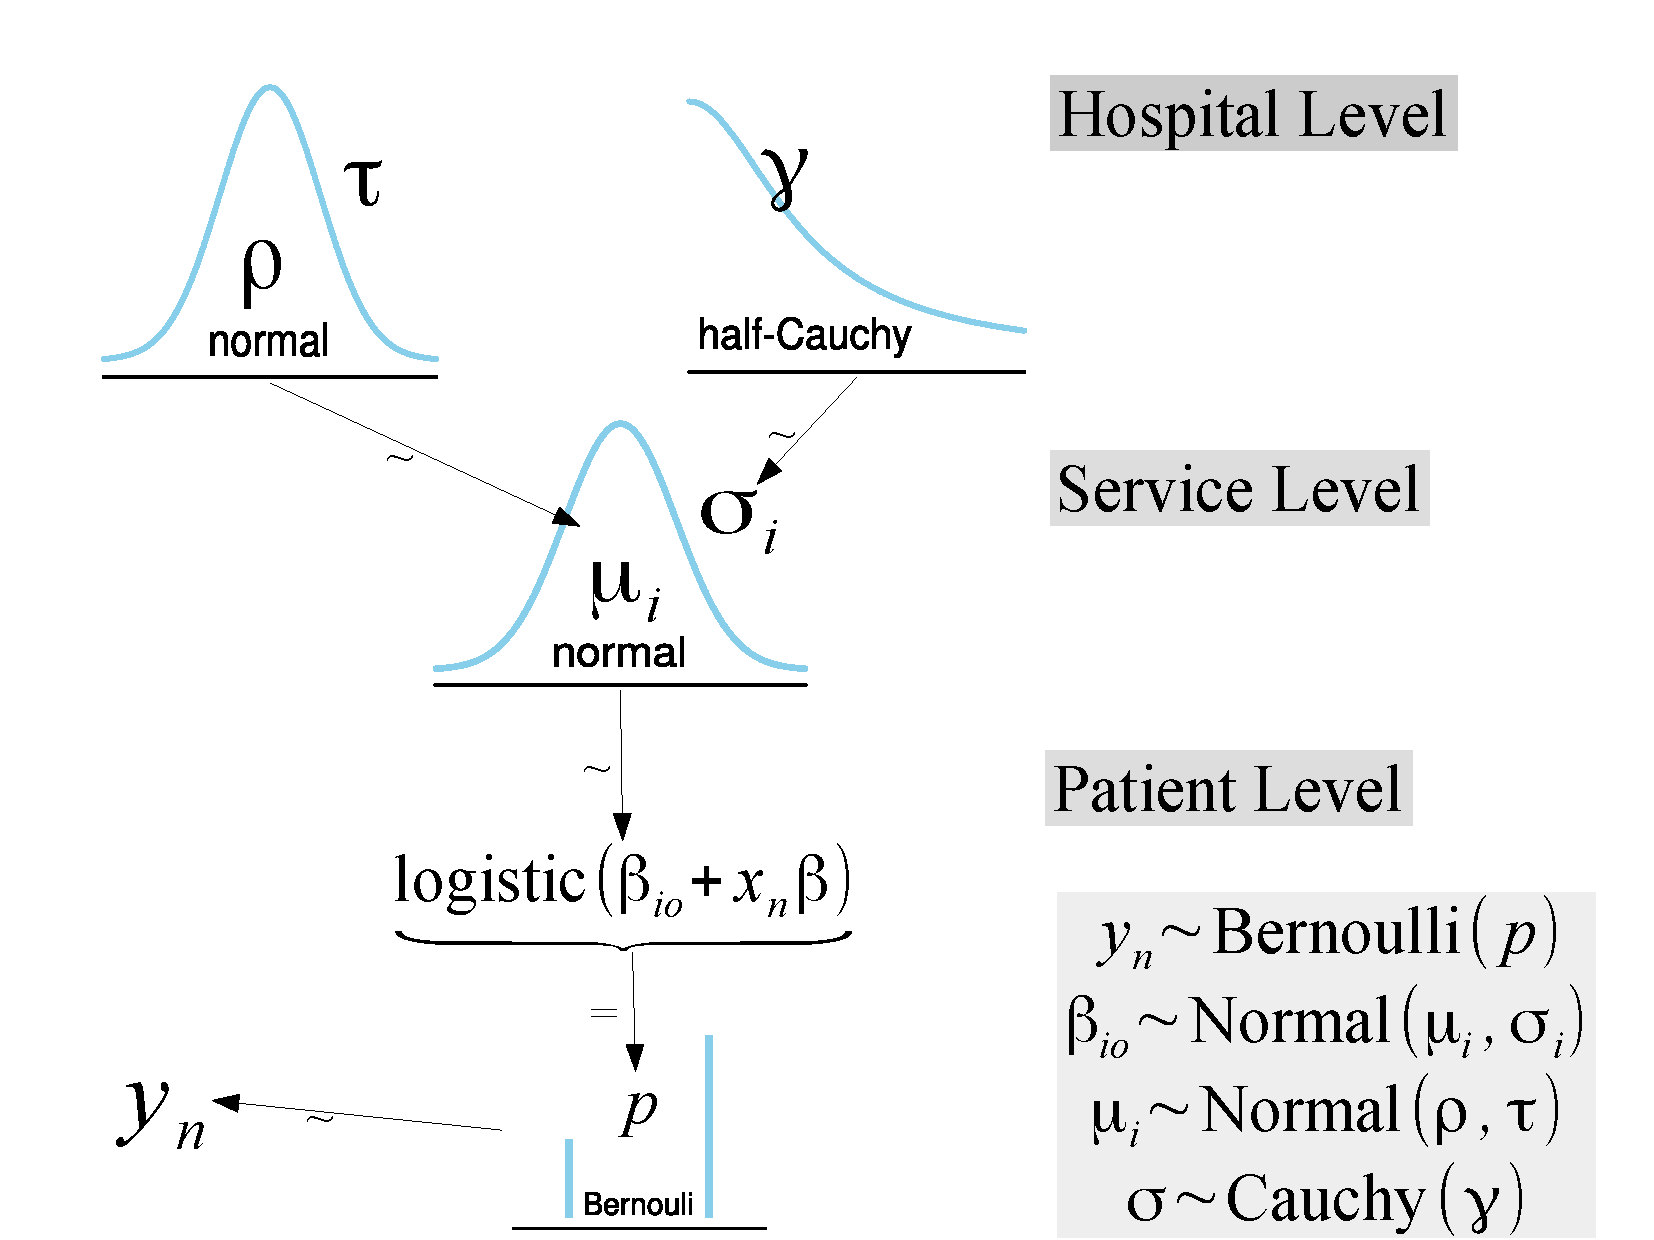
\includegraphics[scale=0.3]{Figures/Distrogram.pdf} 
  \vspace{-20pt}
 \caption{\footnotesize Distrogram to illustrated the hierarchical structure of patient trajectories. Outcome $y_n$ for the $n^{th}$ patient is a boolean indicator predicted by a logistic regression. We allow the patient (random) intercept $\beta_{oi}$ to vary according to the $i^{th}$ medical services the patient is under. The service level mean $\mu_i$ and within-service variance $\sigma_i$ are modeled to vary by hospital. $x_n$ is a vector of patient level predictors, $\beta$ is a vector of regression coefficients.}
 \vspace{-10pt}
 \label{fig:Distrogram}
\end{wrapfigure} 

\subparagraph*{Partial pooling is more efficient for prediction.}
Prediction based on partial pooling outperforms (a) the no-pooling and (b) the complete-pooling approaches, as can be shown mathematically \cite{Efron_1975} or via cross-validation \cite{Gelman-Hill_2014}.  Using the No-pooling approach, we estimate the model for each specific subset of interest separately. But this leads to far too many sub-classifications, thus too small samples in any given subgroup for useful inferences, if we fully explore the complexity and granularity, the richness of the EMR data,. Employing complete pooling or structural modeling constitutes the other extreme of the spectrum, but the implied hard constraints on the coefficients in different groups may lead to bias: we loose information, because we cannot learn from groups where we have more data. We choose the middle ground: Prediction using partial pooling or hierarchical modeling is especially effective for our richly organized EMR data, because the estimate of each individual parameter is simultaneously informed by data from all the other patients in our cohort, improving prediction in particular for subgroups with sparse data. \cite{Gelman_multilevel_2006}. Effron explained this apparent paradox well to non-statisticians in the \href{http://www.nature.com/scientificamerican/journal/v236/n5/pdf/scientificamerican0577-119.pdf}{Scientific American} \cite{Stein_paradox_Scientific_American,Efron_Stein_1977}. 

\subparagraph*{Heterogeneous and incomplete clinical data may limit prediction and implementation.}
Variables with strong predictive power in our model may not be recorded in all patients or may be missing for the time window needed for prediction, limiting development of the prediction algorithm, implementation of the therapeutic interventions and the trial itself. Incomplete data are the hallmark of EMRs. In our data set we find for example that an arterial blood gas (ABG) to assess arterial oxygen tension is often unavailable for the prediction time window, because it was not requested by the physicians. To improve prediction for cases with incomplete data, we can impute the missing data using \textit{multiple imputation}. Likelihood-based mixed effects models for incomplete data give valid estimates \textit{if and only if } the data are ignorably missing; that is, the parameters for the missing data process are distinct from those of the main model for the outcome, and the data are missing at random (MAR) \cite{Rubin_1976}. However, this is an unreasonable assumption for EMRs; in our example, physicians will request ABGs based on the patients respiratory co-morbidity and clinical hypoxia symptoms. Data will not be MAR. Instead, incomplete data will be associated with predictors and outcomes; this could lead to biased imputations.
\begin{wrapfigure}{l}{10cm} 
 \vspace{-10pt}
 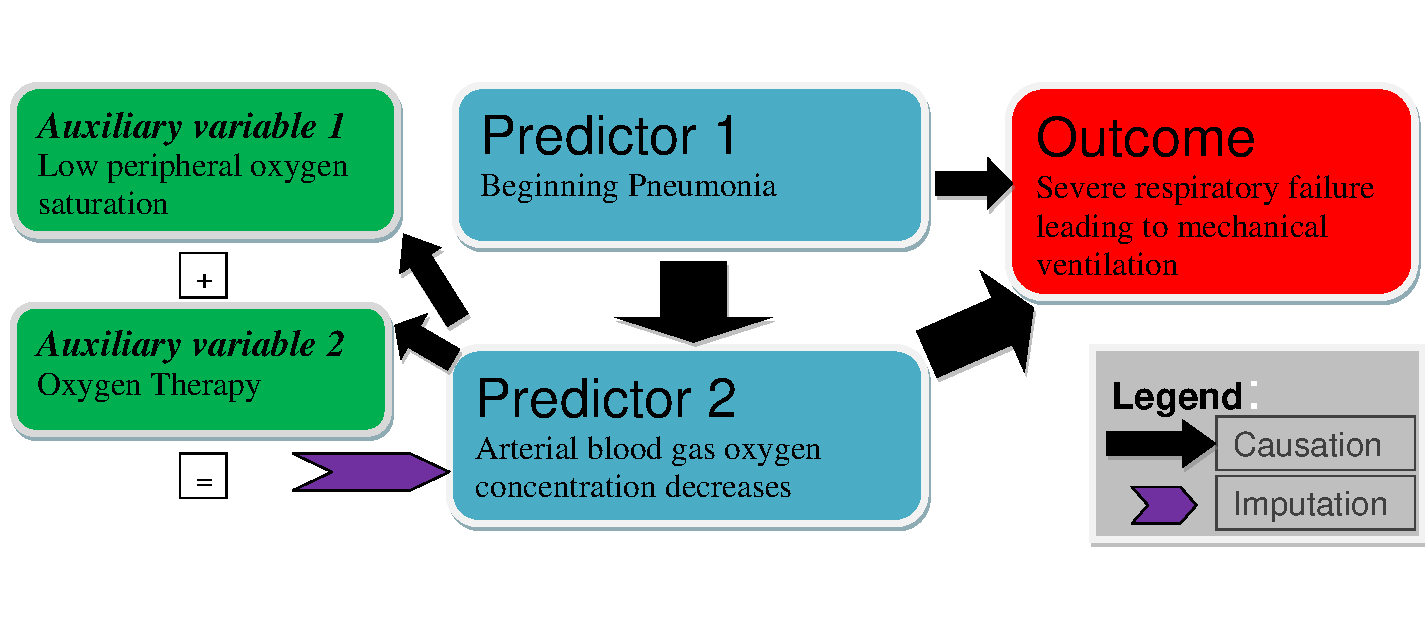
\includegraphics[scale=0.4]{Figures/Bayesian_imputation.pdf}
    \vspace{-20pt}
  \caption{\footnotesize Incomplete data can hinder outcome prediction. We can impute incomplete data from auxilliary information. Pneumonia impairs oxygenation, causing respiratory failure, for example. If arterial blood gases (ABG) are missing, we can impute the arterial $PaO_2$ (oxygen tension) from oxygen therapy and/or peripheral oxygen saturation.  \cite{Hall_25389642}.}
   \vspace{-15pt}
    \label{fig:Imputation_fig}
\end{wrapfigure}
\subparagraph*{Auxiliary data can be used to impute incomplete medical records.} Auxiliary data are additional information available in the form of variables known to be correlated with the missing data of interest \cite{Daniels24571539}. If the physician did not request an ABG, instead peripheral oxygen saturation and or oxygen therapy may be available and could be used to impute the arterial blood oxygen tension [Figure~\ref{fig:Imputation_fig}]. This approach avoids the perils associated with missing at random (MAR) assumptions, when fitting a non-ignorable missingness model \cite{Wang_20029935}. Adding auxiliary variables not included in the main model for multiple imputation, in other words using additional information that is correlated with the missing outcome is an emerging approach to help correct bias \cite{Meng_1994, Collins_11778676, Rubin_1996}, often relying on Bayesian methods \cite{Daniels_2008, Schafer_1997}; joint hierarchical modeling, including auxiliary data to impute incomplete patient records, will improve the prediction model and facilitate the implementation of the prediction algorithm \cite{Hall_25389642}.


\subparagraph*{Seasonal effects and institutional learning can bias risk prediction and can thwart implementation} or imperil the effectiveness of our efforts to mitigate the risks of severe respiratory failure in hospitalized patients. The composition of our hospital population, their co-morbidities and risk profiles change over time, altering which patient characteristics best predict severe adverse respiratory failure and mechanical ventilation. More importantly,  during the implementation phase of previous preventive trials we noted that providers learn, changing their behavior as a result of trial participation. As trials progressed providers implemented previously underutilized interventions more frequently even before they were prompted. We term this effect institutional learning. On the other hand, the transition of junior and senior providers through their training and to other institutions and new personnel joining the staff, may led to lessons learned being forgotten again. Last but not least, respiratory disease is affected by seasonal and secular effects; influenza prevalence for example is seasonal and characterized by major and minor epidemics. Seasons and epidemics will affect the predictive power of any model and hence also alter the risk profile of our patients over time. Institutional culture and individual provider behavior change in response to trials and quality improvements interventions; patient populations change over time. Respiratory patients are plagued by seasonal deterioration. These temporal, seasonal and secular effects will alter the predictors of risk in our model and affect its implementation. We will include these and continuously update our model with new patient data to account for said changes in the risk profile. The integration EMR-triggered prediction and prevention with  institutional learning, secular and seasonal effects as well as data imputations from auxiliary data within one coherent (Bayesian) model is certainly novel, but how can it be implemented in one coherent model? 

\subsection*{B. Innovation}

\subparagraph*{Bayesian hierarchical modeling is groundbreaking in EMR-based prediction,} and particularly suited for joint hierarchical modeling. With their inherent flexibility and robustness \cite{Carlin_1349763,Sutton_2012}, Bayesian hierarchical models may outperform classical models for EMR-based prediction owing to the integration of additional information through "partial pooling" \cite{Gelman_red_2009} and the imputation of incomplete records from auxiliary data. Increases in computer power led to an expansion of applied Bayesian work \cite{Ashby_16947924,Spiegelhalter_11134920}, also in Big Data \cite{Efron_largescale_2013,Yoo_24987556} and more recently in EMR-based prediction \cite{Himes_19261943,Ryynaenen_23496851,Wu_20473190}. \textit{However, we are unaware of any Bayesian hierarchical prediction model based on large EMRs.} 

\subparagraph{A brief introduction to Bayesian inference.} Clinical decision-making is Bayesian \cite{Spiegelhalter_11134920}. Physicians continuously update their preliminary diagnosis with new information. Prior belief $P(A)$ in a diagnosis may be weakened by new laboratory information, leading to an updated diagnosis $P(A|B)$, based on the lab data \cite{Kruschke_22774788, Kruschke_Book_2014}. 
  
\begin{wrapfigure}{l}{.3\textwidth}
\vspace{-10pt}
  \begin{equation}
   \label{eq:Bayes}
P(A \mid B) = \frac{P(B \mid A) \, P(A)}{P(B)}
   \end{equation}
   \vspace{-20pt}
\end{wrapfigure}

According to Bayes' Theorem \ref{eq:Bayes} prior information $P(A)$ is combined with new data, (known as the likelihood) to yield an \textit{updated} estimate for the probability of a hypothesis $P(A)$, given the data $P(B)$ observed, called the posterior distribution $P(A|B)$ \cite{Thomas_Bayes}. Full Bayesian inference is based on priors. Statisticians may object to prior choices (e.g. the cauchy distribution as prior for variance parameters \cite{Gelman_Cauchy_2006} in Figure \ref{fig:Distrogram}).  Principled critique questions the subjectivity of priors. But are not \textit{all} models (frequentist and Bayesian) based on subjective choices \cite{Wagenmakers_Bayesian_v_Freq_2008} (e.g. link function, correlation matrices) or (distributional) assumptions; (Bayesian or classical), these choices need to be reasonable and convincing to the intended audience and should be subjected to sensitivity analysis and model exploration. Combining frequentist with Bayesian thinking may advance Big Data science most \cite{Efron_Bayes_v_Freqentisit,Efron_largescale_2013}. 

\subparagraph*{The computational implementation of Bayesian hierarchical models.}
Bayesian inference for multi-layered models can often not be derived analytically; instead we calculate numerical approximations of the multi-dimensional integrals to obtain the posterior distributions of the parameters of interest. In technical terms, Markov Chain Monte Carlo (MCMC) based Bayesian inference methods sample from a posterior probability distribution after building a Markov chain. MCMC simulation replaces intractable analytical integration with empirical summaries of samples from the posterior distribution \cite{Abrams_9483729}: \textit{Instead of analyzing the odds, we simulate throwing the dice repeatedly.}

\begin{wrapfigure}{l}{.3\textwidth}
 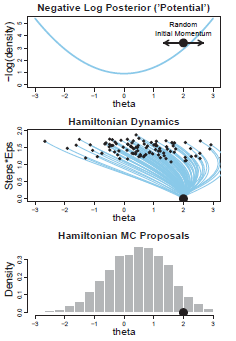
\includegraphics[scale=1]{Figures/Hamiltonian.png}
  \vspace{-20pt}
  \caption{\footnotesize Hamiltonian MCMC uses momentum to optimize the next proposal. The current proposal's higher momentum (black dot) is indicated in the top panel. The middle panel illustrates how random samples are drawn to the mode of the posterior distribution (lower panel) improving convergence and effective sample size. Fig 14 in Kruschke \cite{Kruschke_Book_2014}.}
    \label{fig:Hamiltonian}
 \vspace{- 10 pt}
\end{wrapfigure}

\subparagraph{Pushing the envelope of Bayesian EMR-based prediction,}
we will implement the Bayesian model in parallel in the ultra-fast probabilistic programming language software Stan developed by my co-mentor Dr. Gelman \cite{Stan_Software_2014}. Stan's Hamiltonian Monte Carlo algorithms \cite{Stan_Software_2014} and clever statistical formulation push the boundaries of computability \cite{Gelman-Hill_2014}. For example non-centered parameterization allows sampling in the standardized normal space; this takes full advantage of the faster convergence and higher effective sample size of Stan to overcome computational limitations of Bayesian hierarchical models for Big Data \cite{Gelman-Hill_2014}. Stan  is based on Hamiltonian Monte Carlo (HMC) \cite{Gelman-Hill_2014}, a Markov chain Monte Carlo (MCMC) algorithm \cite{StanislawUlam_1949}, which avoids the sensitivity to correlated parameters that plague many MCMC methods by introducing auxiliary momentum variables \cite{Homan_Gelman_NUTS_2014} as illustrated in Figure~\ref{fig:Hamiltonian}. HMC is dependent on tuning the reciprocal relationship of the crucial parameters step size and desired number of steps. Too low a step size wastes computing power, whereas a step size too large loses efficiency. Stan overcomes this with the No-U-Turn Sampler (NUTS), a recursive algorithm to automate HMC tuning \cite{Homan_Gelman_NUTS_2014}.

\subparagraph*{Analyzing and advancing the practical clinical implementation} of preventive interventions is decisive for outcome improvement and research. Imperfect provider compliance is a major concern also in our PROOFCheck trial, just as non-compliance is a major obstacle to the effective delivery of health care and improved outcomes in general
\cite{Duncan_16710766}. The targeted interventions triggered by our EMR-prediction algorithm will only prevent respiratory failure if our physicians and nurses actually implement them. Improving fidelity of health care providers with evidence based interventions continues to be a challenge and is under-researched \cite{Davis_7650822} and little is known on how to reproduce multi-faceted interventions (specially directed toward providers) to improve clinical outcomes \cite{Campbell_10987780}. As long as we do not understand what drives provider fidelity and patient compliance with the preventive measures proposed to our providers for their high risk patients  \cite{Mittman_15172904}, we ignore the best means to translate widely accepted interventions and new findings of outcomes research into practice \cite{Glasgow_17150029}. We need to understand better what patient and/or provider characteristics hinder compliance with the triggered preventive checklist interventions to ensure care is in accordance with evidence-based best practices.

\subparagraph*{We use a pragmatic trial to investigate provider fidelity.} Pragmatic trials like Dr. Gong's may result in more valid estimates of effectiveness for more realistic health care scenarios \cite{Selby_22824225,Tosh_21842618}; we will use her pragmatic trial data to investigate incomplete fidelity, heterogeneity and difficulty in clinical implementation. An relevant example for PROOFCheck is blood product management: transfusions increase the risk of acute severe respiratory failure with mechanical ventilation \cite{Kenz_24892308}, but implementation of rational transfusion blood product management is still sketchy and very heterogeneous across the nation \cite{Likosky_20488928}. Weiss et al. demonstrated that direct prompting for best practices improves provider compliance in the ICU and outcomes such as duration of mechanical ventilation or length of stay \cite{Weiss_21616996}. We hypothesize that fidelity will be associated with certain provider and patient characteristics; their investigation will allow more focused re-education efforts and adaptation of the checklist implementation. 

\subsection*{Summary of the impact}
Acute respiratory failure in hospitalized patients leading to prolonged mechanical ventilation with the inherent mortality and morbidity constitutes a serious health care challenge. We will tackle this by combining innovative approaches to data imputation with sophisticated hierarchical prediction models to form a near real-time EMR-based clinical decision tool with practical utility in critical care. We use the opportunity to investigate poor provider fidelity a serious and under-researched barrier to outcomes research and the implementation of evidenced-based care. \textit{Our findings will have implications beyond our trial for any clinical research, indeed for the implementation of evidence-based-medicine at large.} Changes in reimbursement give providers a stake in patient outcomes and led to a keen interest in the prediction and prevention of adverse event in hospitalized patients. This project advances hierarchical Bayesian models to implement this paradigm shift in very large EMRs, triggering personalized interventions that deliver outcome improvements. This is novel and has not been attempted to our knowledge. But our impact goes beyond improving morbidity and mortality from respiratory disease in hospitalized patients through improved prediction and prevention, beyond investigating drivers of poor provider compliance. We will develop new methods to impute incomplete electronic medical records from auxiliary data and pioneer Bayesian hierarchical prediction models for large EMR data. Our proposal is unique and novel in its integration of cutting edge methods from clinical, statistical and computer science to fully realize the promise of Big Data in medicine.

\subsection*{C. Approach}
My research project will be closely aligned with my mentor's NIH-funded pragmatic two phase trial. Aim 1 will utilize the processed data of APPROVE to improve the prediction model and Aim 2 will use the data from the implementation of PROOFCheck to investigate fidelity of the providers with the EMR-triggered interventions.

\subsubsection*{Aim 1: To improve incomplete data imputation and early prediction of acute respiratory failure.}


\textit{Hypothesis: The integration of auxiliary data imputation and multi-level Bayesian modeling will improve prediction of severe respiratory failure in hospitalized patients compared to classical statistical approaches.}


\subparagraph*{For specific aim 1a,} we will build a pragmatic EMR-based hierarchical Bayesian model to predict a composite outcome [mechanical ventilation prolonged beyond 48 hours or death] in hospitalized adult and compare our Bayesian approach with the existing frequentist algorithm used by Dr. Gong in her pragmatic trial.

\subparagraph*{Population:}
We will include all adults patients, admitted to the Montefiore Medical Center during APPROVE, excluding only those who are chronically ventilated at home or who have Do not resuscitate orders at the time of hospital admission. APPROVE is Dr. Gong's prospective observational cohort study underway at Montefiore and the Mayo Clinic Rochester, described in detail under Significance; we will build our Bayesian hierarchical model based solely on Montefiore patients. We will divide the cohort into separate fitting and validation set.

\subparagraph*{Predictors:}
We will consider time-invariant and time-variant demographic and clinical data for inclusion as independent predictors in our model. Examples for demographics are gender, age, medical service or ward, examples for physiological and clinical predictors are heart rate, blood pressure or lab tests. Certain predictors will require summary aggregations and (logarithmic) transformations to induce variance stability.

\subparagraph*{Outcomes:}
Our primary outcome will be acute respiratory failure requiring mechanical ventilation longer than 48 hours, specified as positive for (a) mechanical ventilation lasting longer than 48 hours or (b) mechanical ventilation lasts less than 48 hours, but the patient died within 96 hours of the calculated score. Patients that are not on prolonged ventilation within 96 hours or discharged alive from the hospital will be considered negative.

\subparagraph*{Bayesian hierarchical modeling to reflect the nested structure of health care.}   
We will build a Bayesian hierarchical multivariate logistic regression model of time-invariant and time-variant demographic, clinical and administrative variables. Our Bayesian hierarchical modeling will represent the multi-level nested structure of current health care, with levels for medical or surgical service the patient is under, the floor or ward where the patient is cared for, the institution the patient is admitted to. We may also consider other random effects for example for co-morbidity and other time-invariant patient specific descriptors. We illustrate this nested structure in a simplified logistic model with hierarchical levels for patient, service and hospital, analogous to Figure \ref{fig:Distrogram}. 

\begin{wrapfigure}{l}{.5\textwidth}
\vspace{-10pt}
 \begin{equation} \label{eq:patientlevel}
 y_{n} \sim bernulli \Big(inv\_logit (\beta_{0} +\beta_{1} * PaO_2) \Big)
 \end{equation}
\vspace{-25pt}
\end{wrapfigure}

\subparagraph*{Patient level (\ref{eq:patientlevel})}
On the left, we model at the patient level, the probability that the $n^{th}$ patient will develop the dichotomous event $y_n$, (acute respiratory failure requiring prolonged mechanical ventilation), using say arterial oxygen tension $PaO_{2}$ as one predictor in a simple logistic regression model. However, patients are typically assigned to different services. Pulmonary service patients may have a lower baseline $PaO_2$, while surgical patients tend to have normal lung function. 

\begin{wrapfigure}{l}{.5\textwidth}
\vspace{-10pt}
\begin{equation} \label{eq:servicelevel}
 \beta_{0i} \sim Normal (\mu_i , \sigma_{i}); \beta_{1i} \sim Normal (\kappa_i, \sigma_{\beta_1i})
\end{equation}
\vspace{-25pt}
\end{wrapfigure}

\subparagraph*{Service level (\ref{eq:servicelevel})}
On the left, we develop our hierarchical model further to allow random intercepts $\beta_{0i}$ modeling that the average  $\mu_i$ baseline arterial oxygen tension ($PaO_2$) may vary between a given medical $service_i$ and another say surgical $service_{i+1}$. Analogously, smaller changes in $PaO_2$ may be indicative of respiratory deterioration in a certain medical $service_i$, compared to a surgical $service_{i+1}$, where only a larger drop in arterial oxygen tension effectively predicts outcome. We may allow the regression coefficient for the slope $\beta_{1i}$ to vary around different mean slopes $\kappa_i$ at the service level $i$. 

\begin{wrapfigure}{l}{.5\textwidth}
\vspace{-10pt}
\begin{equation} \label{eq:hosptiallevel}
 \mu_i \sim Normal(\rho_, \tau); \sigma_{\beta_{1i}} \sim Cauchy(\gamma)
\end{equation}
\vspace{-25pt}
\end{wrapfigure}

\subparagraph*{Hospital level (\ref{eq:hosptiallevel})}
Even within one academic institution, some (city) hospitals may cater to a economically more disadvantages population, which is sicker on average. To reflect this, we may  model the mean intercept $\mu_i$ for the services hierarchically at the hospital level. Analogously, patients may differ very much between services in one hospital, leading to a larger variance $\sigma_{\beta_{1i}}$, while another hospital may have a more homogeneous patient population leading to a more narrow distribution of regression parameters; we can model this \textit{variation} $\sigma_{\beta_1}$ of the mean slope $\mu_1$ within services at a given hospital to capture the variability of $PaO_2$'s predictive effect. We will compare our model to the classical frequentist prediction model currently build by Dr. Gong's statistical team.

\subparagraph*{Data Acquisition}
Data will be abstracted from a clinical data warehouse(see Environment and Resources). A multi-prong approach for capturing complete, longitudinal data in real-time, near real-time, or asynchronously from the EMR replica will be used. Montefiore Enterprise Clinical Research Management Systems will provide secured electronic data capture tools to streamline, quality control, normalize, and manage data collection and entry efforts. A fully de-identified, study specific database will be compiled for model development and validation.
\begin{wrapfigure}{l}{.35\textwidth}
\vspace{-20pt}
\begin{equation} \label{eq:predictivecheck}
 p(y^{rep}|y)  = \int \! p(y^{rep}|\theta) p(\theta|y) \, \mathrm{d}\theta 
\end{equation}
\vspace{-20pt}
\end{wrapfigure}
If our model is a good fit, then data generated by the model using the estimated parameters should have a distribution similar to the original data we observed. We illustrate this idea behind posterior predictive checking \cite{Gelman_predictive_2000} in Figure~\ref{fig:posteriorpredictivecheck}, generated in our software package shinyStan \cite{shinystan-software:2015}:

\subparagraph*{Model checking}
We will look at auto-correlation, trace-plots and calculate the Gelman and Rubin's MCMC Convergence Diagnostic $ \hat{R}$ to evaluate the the convergence of our Markov chain Monte Carlo (MCMC) simulations using \href{http://andrewgelman.com/2015/03/02/introducing-shinystan/}{shinyStan}, the interactive visual application to graphically explore hierarchical models, we developed \cite{shinystan-software:2015}. Others reviewed shinyStan's installation and utility on \href{https://www.youtube.com/watch?v=X31xqNHcvQs}{YouTube}. In evaluating our Bayesian model's predictive performance, exploratory graphical \cite{Gelman2004posteriorpredictivechecks} and confirmatory formal posterior predictive assessment using discrepancies \cite{GelmanMengStern1996} will complement each other to compare the patient test set to simulated replications from our fitted hierarchical Bayesian model. As a simple example, for each draw of the estimated parameter $\theta$ from the posterior $p(\theta|y)$ we simulate data $y^{rep}$ from the posterior predictive distribution $ p(y^{rep}|y) $. Using the simulations of $y^{rep}$ we can make various graphical displays comparing our observed data to the replications. As a more sophisticated approach we will graphically contrast the vector test statistics $T(y)$ versus replicated data $T(y^{rep})$ to detect a potential misfit of model to data \cite{Gelman2004posteriorpredictivechecks,Buja1999inference} Analogously, we will use predictive validation to adjust for overfitting of our model and perform a sensitivity analysis of our priors on key model parameteters \cite{Gelman-Hill_2014,Gelman_predictive_2000}.

\subparagraph*{Model comparison}

\begin{wrapfigure}{R!}{.3\textwidth} 
 \vspace{-20pt}
 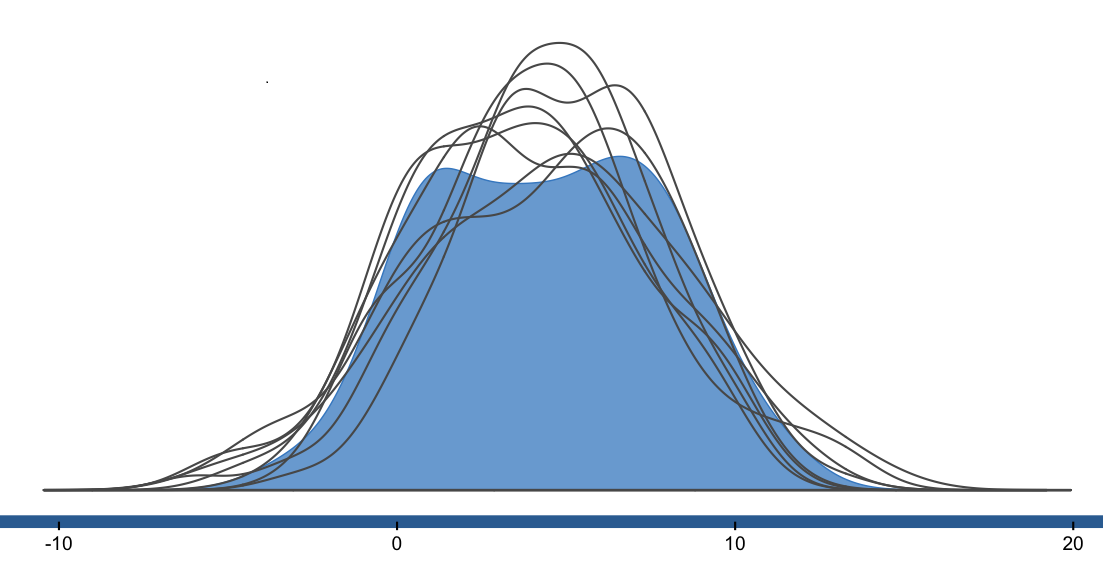
\includegraphics[scale=0.2]{Figures/posteriorpredictivecheck.png} 
  \caption{\footnotesize Exploratory posterior predictive check with our software shinyStan \cite{shinystan-software:2015}: The most basic exploratory graphic \cite{Gelman2004posteriorpredictivechecks} is simply a comparison of the entire data set (here the distribution of observed outcomes shaded in blue) to a reference distribution, (distributions of simulated outcomes shown as thin lines). An approximate match suggest a reasonable fit.}
  \label{fig:posteriorpredictivecheck}
  \vspace{-20pt}
\end{wrapfigure}

We will assess the plausibility of our posited hierarchical model and its assumptions \cite{Gelman_predictive_2000,GelmanMengStern1996} and will compare it to the alternative classical model by Dr. Gong (based on a non-nested much simpler model \cite{Herridge_12594312}). As a simple approach, we will perform a nonparametric comparison of areas under the curve (AUC) of the correlated receiver operating characteristics (ROC) curves \cite{DeLong_3203132} to assess their respective predictive performance \cite{Newcombe_22890972,Wu_20473190}, in other words to investigate if the hierarchical modeling improves prediction of acute severe respiratory failure over the simpler classical model used by Dr. Gong. We will compare the models based on a different test set from the same population, to avoid biasing the comparison in favor of our more complicated, (possibly overfitted) hierarchical model. Cross-validation is widely used to compare statistical models for estimating out-of-sample prediction error \cite{Vehtari_12396570}. However, in our case, we operate on the limits of computability and repeatedly fitting our Bayesian hierarchical model to leave-one-out samples, could be computationally too expensive \cite{Gelman_Aki_2014predictive}. Besides, for multi-level data, leaving partitioning the data for cross-validation should probably consider the hierarchical structure itself; indeed, cross-validation may not always be a sensitive instrument for model comparison \cite{wang_predictive_2014}. We will also explore the predictive information of our hierarchical model using posterior predicitve simulations and realized discrepancies \cite{Gelman_Aki_2014predictive,Gelman_predictive_2000,GelmanMengStern1996}. In parallel sampling \cite{Congdon_modelcomparison_2005}, we will compare our Bayesian Model to the classical simpler algorithms using the minimum $\chi^{2}$ discrepancy, essentially equivalent to the classical goodness-of-fit test statistic \cite{GelmanMengStern1996}. For additional validation, we will train our model with patient data from other participating institutions (Mayo Clinic Rochester and Florida) and test if our model outperforms the classical prediction models even in other ecological settings (say Mayo Clinic Rochester) or if the classical model is based on data from all institutions.

\subparagraph*{Technical approach}
Boolean combinations of data matching and natural language processing of the prediction algorithms will be used to scan a real time copy of the hospital's clinical and administrative data including demographic, monitoring, pharmacy, laboratory, and physician notes for risk factors and physiological abnormality. The rule engine (implemented in Java) will send out the alert to providers.

\subparagraph*{For specific aim 1b,} we develop new Bayesian data imputation algorithms for missing clinical data using auxiliary data and we identify auxiliary measure properties (ceiling, floor and threshold effects). Missing data are a characteristic limitation of large electronic medical records and may bias our prediction model \cite{Dean_19279318}. Electronically medical records measurements not updated 24 hours earlier than the selected start time will be considered missing;  as an illustrative example, we formulated a simplistic model illustrated in [Figure~\ref{fig:Imputation_fig}]. We predict acute respiratory failure, the dichotomous compound outcome $Y$ in Equation \ref{eq:Impute1}; we integrate this with a model for latent arterial oxygen tension $\Omega$ in a logistic regression model in Equation \ref{eq:Impute2}, contingent on having $PaO_{2}$ from an arterial blood gas (ABG) or not. Nota bene, ABGs will certainly not be missing at random, but contingent on the $PaO_2$ value and respiratory outcome $Y$. 

\begin{wrapfigure}{L!}{.57\textwidth} 
\vspace{-25pt}
\begin{align} \label{eq:Impute1}
Y \sim Binom(\mu, n); \mu = inv\_logit(\beta_{0} + \beta_{1} * \Omega) \\ \label{eq:Impute2}
\Omega =  I(observed = true) * PaO_{2}   +   I(observed = false) * \delta  \\ 
\delta \sim Normal(\theta, \tau); \theta = \gamma_{0} + \gamma_{1}* O_{2} Sat + \gamma_{2} * O_{2} Therapy \label{eq:Impute4}
\end{align}
\vspace{-35pt}
\end{wrapfigure}

\vspace{5pt} If the $PaO_{2}$ from the ABG is observed, we will use it to predict the outcome $Y$. If no ABG was obtained, we impute the latent oxygen tension $\Omega$ with a regression model from the auxiliary data  $O_{2}$ Saturation and $O_{2}$ therapy in Equation \ref{eq:Impute4}. We will identify the auxiliary measure properties, ceiling and floor and potential threshold effects effects, test the imputations against manually verified data and published algorithms and compare them to  simple and multiple imputation strategies in Dr. Gong's trial \cite{Huntington_16311133,Sloan_15027501}.  

\subsubsection*{Aim 2: To model temporality (institutional learning, seasons) and investigate provider compliance.}
To focus education efforts and improve implementation of preventive or therapeutic measures, we will investigate predictors of provider behavior. To most closely reflect the realistic situation of actual academic and community medical delivery settings, we need to take temporal and seasonal changes into account. 
  
\paragraph*{For specific Aim 2a,} we will investigate provider compliance with the individual components of the checklist. During the second phase (PROOFCheck) of Dr. Gong's pragmatic trial, providers of a patient identified as high risk by the frequentist prediction algorithm will be prompted electronically to implement concrete preventive and corrective measures from a list of widely accepted interventions. During roll-out, providers receive targeted education on prevention and best practice. During PROOFCheck, an interactive notification algorithm will suggest to the physicians patient specific interventions from the checklist to the clinicians via an electronic clinical interface. 

\paragraph*{Prediction of adverse events is useful only if followed by effective preventive action. } We will use data from PROOFCheck, the second phase of Dr. Gong's pragmatic trial to analyze provider compliance (fidelity) with the proposed interventions. We will investigate which provider and patient characteristics predict compliance with which components of the intervention checklist to identify drivers of poor provider fidelity. Results will inform our compliance retraining for PROOFCheck in which I will actively participate during my second year.

\paragraph*{Population:} 
Hospitalized adults identified by the APPROVE algorithm  as high risk and intubated patients will be included in Dr. Gong's PROOFCheck. PROOFCheck will limit recruitment to wards found to have higher prevalence of severe adverse respiratory events during the first phase of Dr. Gong's trial (APPROVE). Patients chronically ventilated at home or who have DNR, will be excluded. I will include all data from all participating centers. We anticipate enrollment of 12,000 patients over 4 years.

\subparagraph*{Outcomes,exposures and predictors:}
My primary outcome will be provider compliance, a dichotomous event, defined as positive if the provider ordered the prompted preventive intervention. In order to measure and demonstrate compliance with the checklist, near real time (same day) transaction logs evidence for compliance will be recorded electronically. We will consider time-invariant and time-variant provider and patient demographic and clinical data.  Two hypothetical examples of provider and patient demographics as predictors fidelity: (1) junior residents may be less comfortable with stricter blood transfusion triggers compared to seasoned physician assistants; (2) providers fidelity with evidence based treatment recommendations may be contingent on patient gender, say for heart failure \cite{Cook_25714825}, likely an important predictor of respiratory failure in APPROVE. Time-variant patient characteristics (e.g. lab values) could determine provider fidelity; for example borderline blood hemoglobin concentration may influence compliance with PROOFCheck blood transfusion recommendations.

\subparagraph*{Study design and model building}
This is a prospective observational cohort study to investigate sustained provider fidelity with EMR-triggered preventive interventions in PROOFCheck, Dr. Gong's pragmatic multicenter trial. We will build a Bayesian hierarchical multivariate logistic regression model of time-invariant and time-variant demographic, clinical  and administrative variables, with levels for service, ward and institution, analogously to aim 1; the hierarchical structure is to reflect certain biases and attitudes ingrained in certain specialties or hospitals, which may lead to different associations between provider and patient characteristics and fidelity with treatment alerts, e.g. service-specific reluctance to use triggers to minimize blood cell transfusion \cite{Goodnough_23706801}. 

\paragraph*{For specific Aim 2b,} to reflect changing risk profiles over time, we will adjust our Bayesian model to update continuously with new incoming patients and adapt our model to include temporal effects, like institutional learning, seasonal or endemic phenomena. Seasonal changes could for example be modeled by adding another level above the hospital level to our patient-service-hospital hierarchy illustrated in Figure \ref{fig:Distrogram}. This would allow the hospital level mean to vary over time to reflect increases in the severity and prevalence of chronic obstructive pulmonary disease in the winter or to smooth over differences in annual flu prevalence.

\subsubsection*{Preliminary work and feasibility of our research plan }

\begin{figure}[h]
 \vspace{-20pt}
 \centering
   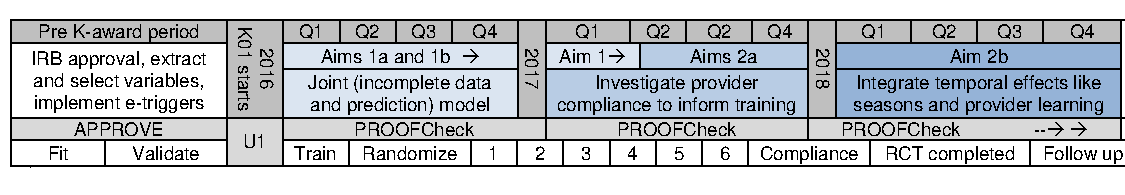
\includegraphics[scale=1]{Figures/Timeline.pdf}  
 \vspace{-30pt}
 \caption*{\footnotesize \textbf{Timeline}, detailing quarterly progress through the K01 training period: My research plan is well aligned with APRROVE and PROOFCheck, my mentor's trial. Time consuming preliminary work (IRB approval, computerized data collection and cleaning, aggregation and standardization, identification of important predictors of respiratory failure) is already well under way. Cluster randomization [for hospital 1-6] begins soon after my K01 starts. Aim 1 will have considerable overlap into the second year, when concurrent fidelity analysis will inform compliance retraining for PROOFCheck. Rich data will sustain my final integration of temporal effects in the model.}
  \vspace{-10pt}
  \label{fig:Timeline}
 \end{figure}
 
Successful execution of my research plan is facilitated by its integration in my mentor's trial, illustrated above. We have already abstracted data from 68,000 patients from Monte and Mayo for derivation and validation for APPROVE. The computability of our Bayesian model hinges on its effective computational implementation. My co-mentor, Dr. Gelman is personally invested in the realization of cutting-edge Bayesian models through our allied R01 research project. Several standalone components of my research proposal will lead to high impact publications: missing data imputation using auxiliary data is novel, as is the analysis of poor provider compliance. 

\subsubsection*{My research is well aligned with NIH funding opportunities, institutional priorities and emerging paradigms}
Together with my mentors Drs. Gong, Gelman and Hall, we are working on an related R01 application to further develop Bayesian computational algorithms, using Dr. Gong's trial as use case. Culminating a PhD, my K01 training will give me the competitive edge to lead similar multi-disciplinary NIH applications as early stage principle investigator. I am particularly interested to extend our Bayesian tools to the "Perioperative Surgical Home" \cite{Vetter_24781579}.


%----------------------------------------------------------------------------------------
%	BIBLIOGRAPHY
%----------------------------------------------------------------------------------------

\newpage

\nobibliography{K01_bibliography_24Feb15} % to not print a bibiography at the end.
% \bibliography{K01_bibliography_24Feb15} % the file name cannot contain spaces
\bibliographystyle{nihunsrt} % Use the custom nihunsrt bibliography style included with the template

%----------------------------------------------------------------------------------------

\end{document} 
